\documentclass[12pt]{article}
\setlength{\textwidth}{17cm}
\setlength{\textheight}{24cm}
\setlength{\topmargin}{-2cm}
\setlength{\footskip}{1cm}
\setlength{\evensidemargin}{0cm}
\setlength{\oddsidemargin}{0cm}
\setlength{\parindent}{1.5em}


\usepackage{allrunes}
\usepackage{amsmath}
\usepackage[magyar]{babel}
\usepackage[T1]{fontenc}
\usepackage[utf8]{inputenc}
\usepackage{fixltx2e}
\usepackage{multirow}

\usepackage[hyphens]{url}
\usepackage[unicode,colorlinks=true,breaklinks]{hyperref}
%\usepackage[dvips]{hyperref}
%should display links, but it does not work with \H accent
%and formulas in section titles

\hypersetup{colorlinks,linkcolor=blue,urlcolor=magenta,citecolor=magenta}
%Breaks long url`s in text, while keeping it one link:

\usepackage{amsfonts}
\usepackage{amsthm}
\usepackage{amssymb}


\theoremstyle{plain}
\usepackage{graphicx}

%\usepackage{gensymb}
\usepackage{float}

% For bra-ket notation
\usepackage{braket}

%% New commands
\newcommand{\dd}{\textrm{d}}

\bibliographystyle{unsrt}




\begin{document}
\title{14. tétel \\ Számítógépes hálózatok}
\author{Bulatovic Nikola}

\maketitle

\begin{abstract}
    A hálózati adatátvitel fizikai rétege, ethernet, az optikai adatátvitel módszerei. Vezeték nélküli hálózatok. IP hálózatok, végpontok, kapcsolók, útválasztók, tűzfalak, IP cím, TCP, UDP, DNS, NAT. Sávszélesség, sorban állás, torlódás. Hálózati topológiák. Adattitkosítás. \par
    Ez a tétel főként a \textit{Számítógépes alapismeretek} kurzus és a hozzá tartozó jegyzetek alapján készült \cite{szamalap1, szamalap2}. A felhasznált irodalom közt szerepel a témakör egyik alapműve \cite{tanenbaum}, illetve egyéb forrás is \cite{magyar}. A tételben azok a témák lettek részletesebben kidolgozva, amelyek az említett kurzuson szerepeltek. A további témák, melyek valamilyen egyéb speciális kurzuson hangoztak el (sorbanállás/torlódás, adattitkosítás) csak tömören, egy átfogó képet adva kerülnek bemutatásra a továbbiakban. 

\end{abstract}

\tableofcontents
\newpage

\section{Bevezetés - számítógépes hálózatok}

A számítógépes hálózatok egymással összeköttetésben lévő, különálló számítógépek (hostok) együttese. Az ilyen számítógépes hálózatok előnyei:
\begin{itemize}
\setlength\itemsep{-0.2em}
    \item adat-,
    \item erőforrás-,
    \item terhelésmegosztás, 
    \item megbízhatóságnövelés, stb.
\end{itemize}{}
Természetesen vannak hátrányai is, mint pl.:
\begin{itemize}
\setlength\itemsep{-0.2em}
    \item Adatbiztonsági problémák (az adatokat olyanokkal is megoszthatjuk, akikkel nem szeretnénk).
    \item Vírusok gyorsabb terjedése, stb.
\end{itemize}{}

\par
\medskip
Ahogy később látni fogjuk, a hálózatoknak sokféle mérete, alakja, formája lehetséges. Ezeket általában összekapcsolják egymással, egy nagyobb hálózat kialakításának céljából. Erre a legismertebb példa az internet. 
\par
\medskip
Megjegyzés: habár jelentős átfedés van közöttük, a számítógép-hálózat és az elosztott rendszer két különböző fogalom. Az elosztott rendszerben a független számítógépek együttese egyetlen koherens rendszernek tűnik a felhasználói számára, melynek megvalósításáért egy, az operációs rendszerre épülő szoftverréteg felel. Erre példa a világháló (worl wide web). Egy számítógép-hálózatban ez a koherencia, az egységes modell és a közös szoftver hiányzik. Az elosztott rendszer lényegében egy olyan szoftverrendszer, amely egy hálózatra épül rá. A szoftver biztosítja a nagyfokú egységességet és az átláthatóságot. Ebből kifolyólag a különbség egy számítógép-hálózat és egy elosztott rendszer között sokkal inkább a szoftverben, mint a hardverben van.

\section{Hálózatok csoportosítása méret, topológia alapján}

A számítógép-hálózat általában egy térben jó körülhatárolható területen elhelyezkedő gépeket köt össze. A hálózatokat csoportosíthatjuk aszerint, hogy mekkora területen helyezkednek el az egymással összekapcsolt hostok (\ref{fig:size}. ábra):
\begin{itemize}
    \item LAN (Local Area Network): Legkisebb hálózatok. A hostok általában egy teremben, épületben helyezkednek el.
    \item MAN (Metropolitan Area Network): Nagyváros méretű, vagy néhány 10 km-es sugarú körben elhelyezkedő hálózatok.
    \item WAN (Wide Area Network): Széles, nagykiterjedésű hálózatok, esetleg földrészek között.
    \item GAN (Global Area Network): Az egész világot átölelő hálózat, mint például internet.
\end{itemize}{}

\begin{figure}[H]
    \begin{center}
    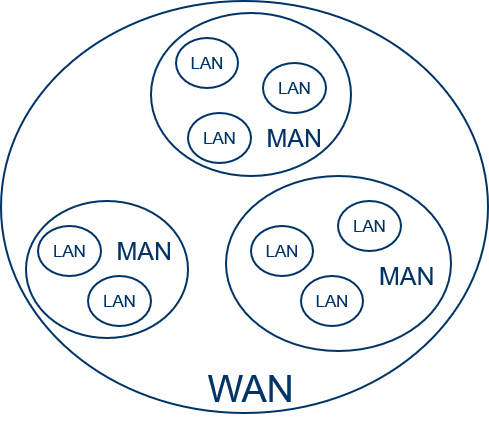
\includegraphics[width=0.33\textwidth]{media/size.png}
    \caption{\textbf{Hálózatok csoportosítása területi kiterjedés alapján.}} 
    \label{fig:size}
    \end{center}
\end{figure}

A számítógép-hálózatokban a hostok és az azokat összekötő kommunikációs csatornák kapcsolódásának rendszerét topológiának nevezzük.  A legfontosabb hálózati topológia típusok (\ref{fig:top}. ábra): busz, gyűrű, fa, csillag, hópehely, teljesen összefüggő.

\begin{figure}[H]
\centering
    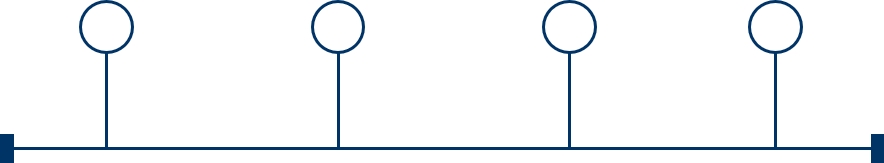
\includegraphics[width=0.3\textwidth]{media/bus.png}
    \hspace{0.75cm}
    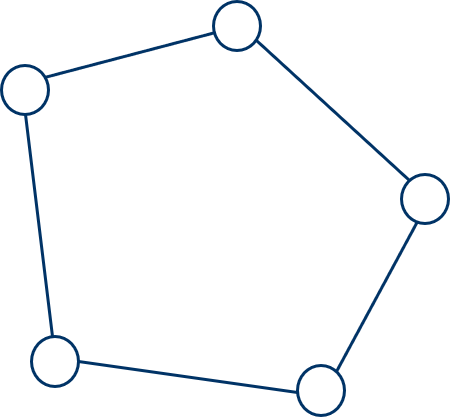
\includegraphics[width=0.3\textwidth]{media/gyuru.png}
    \vspace{1.5cm}
    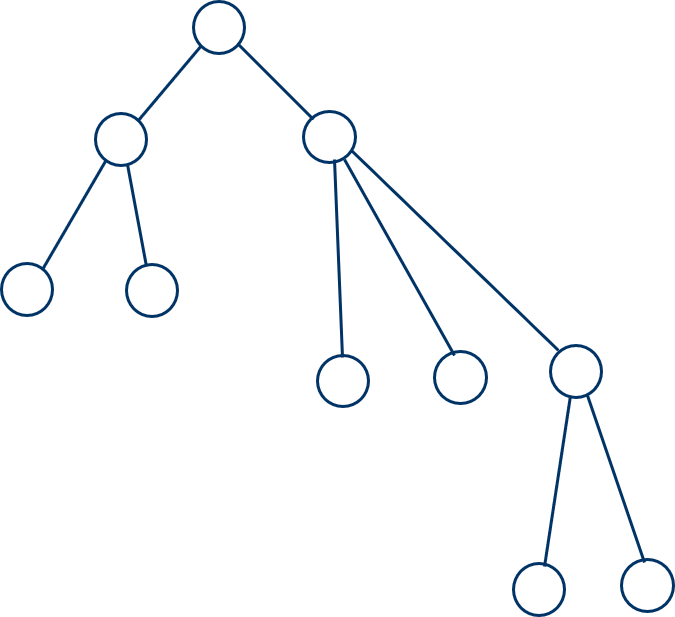
\includegraphics[width=0.3\textwidth]{media/fa.png}
    \hspace{1cm}
    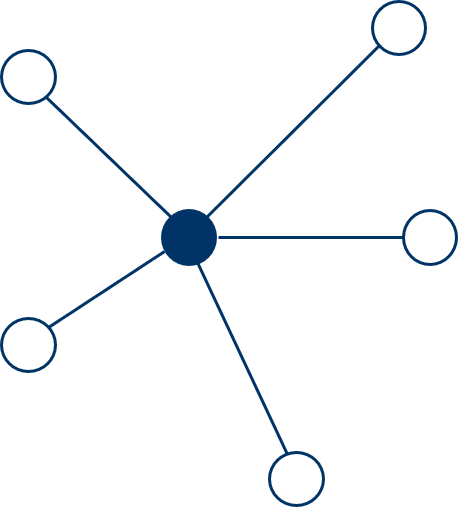
\includegraphics[width=0.3\textwidth]{media/csillag.png}
    \vspace{1.5cm}
    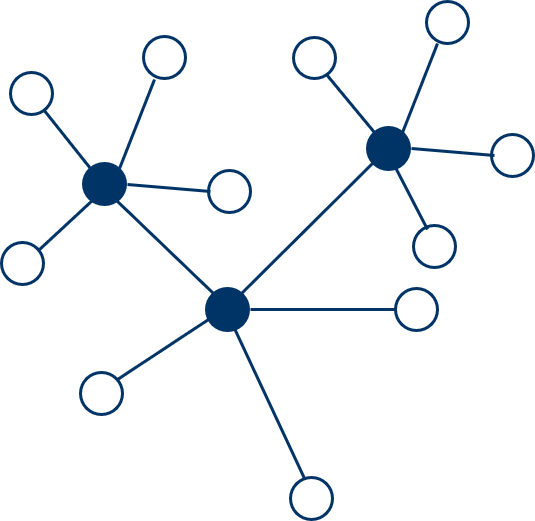
\includegraphics[width=0.3\textwidth]{media/hop.png}
     \hspace{1cm}
    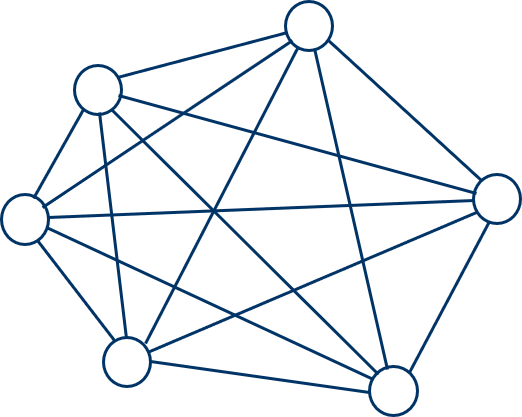
\includegraphics[width=0.3\textwidth]{media/telj.png}    
    \caption{\textbf{Hálózati topológiák.} A bal felső sarokból jobbra indulva: busz, gyűrű, fa, csillag, hópehely, teljesen összefüggő.} 
    \label{fig:top}

\end{figure}

\section{Hálózati architektúrák}

A hálózat tervezés bonyolultságának csökkentése érdekében, a legtöbb hálózatot úgy alakítják ki, hogy azok egymásra épülő rétegeket vagy szinteket (layer, level) képezzenek. A rétegek száma, elnevezése, tartalma és feladata más és más a különböző hálózatokban. Minden réteg célja az, hogy bizonyos szolgáltatásokat (service) nyújtson a felette elhelyezkedő rétegeknek, miközben elrejti előlük a szolgáltatások tényleges megvalósításának részleteit. Két számítógép esetén csak az azonos szintű rétegek kommunikálnak egymással (\ref{fig:layer}. ábra). E kommunikáció szabályrendszere a protokoll. A protokollok és a rétegek halmazát nevezzük hálózati architektúrának.


\begin{figure}[H]
    \begin{center}
    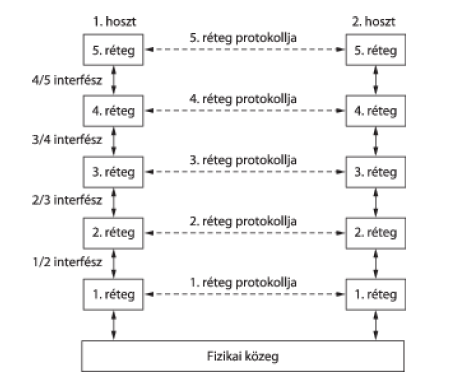
\includegraphics[width=0.5\textwidth]{media/layer.png}
    \caption{\textbf{Rétegzett hálózati architektúra.}} 
    \label{fig:layer}
    \end{center}
\end{figure}

\subsection{Fizikai réteg - Ethernet}

A valóságban az egyik gép n-edik rétegéből az adatok nem közvetlenül jutnak át egy másik gép n-edik rétegébe, hanem valamilyen vezérlőinformációval kiegészítve mindegyik réteg közvetlenül az alatta levőnek továbbítja az adatokat (az ún. interfacen keresztül) egészen addig, amíg azok a legalsó rétegig el nem jutnak. \\ \par
A hálózati architektúrák megvalósítására többféle elméleti modell létezik pl.: ISO/OSI vagy TCP/IP. Ezek közös tulajdonsága, hogy a legalsó réteg az ún. fizikai réteg (physical layer), ahol a tényleges kommunikáció zajlik a host-ok között. \\ \par
A legelterjedtebb ilyen hálózati technológia az Ethernet. Szinte minden hálózatra köthető eszköznél használható, ehhez egy megfelelő hálózati kártya szükséges. A szabvány folyamatosan fejlődik, az átviteli közegtől függően nagy sebességű adatátvitelre képes. A legfontosabb hálózati architektúrák fizikai rétegét ez a protokoll definiálja, így a gyakorlatban a fizikai adatátviteli réteg szinonimájaként használják.
\\ \par
A fizikai réteg feladata az, hogy továbbítsa a biteket a kommunikációs csatornán. A rétegnek biztosítania kell azt, hogy az egyik oldalon elküldött 1-es bit a másik oldalon is 1-esként érkezzen meg, ne pedig 0-ként. Ez a réteg tipikusan olyan kérdésekkel foglalkozik, hogy mekkora feszültséget kell használni a logikai 1, és mekkorát a logikai 0 reprezentálásához, mennyi ideig tart egy bit továbbítása, az átvitel megvalósítható-e egyszerre mindkét irányban, miként jön létre az összeköttetés, hogyan bomlik le, ha már nincs szükség rá, hány érintkezője van a hálózati csatlakozóknak, mire lehet használni az egyes érintkezőket stb. A tervezési szempontok itt főleg az interfész mechanikai, elektromos és eljárási kérdéseire, valamint a fizikai réteg alatt elhelyezkedő fizikai átviteli közegre vonatkoznak.
\\ \par
A fizikai átviteli közegek csoportosítása:
\begin{itemize}
\item Vezetékes (\ref{fig:vez}. ábra):
\begin{itemize}
\item[-] Csavart érpár: Két szigetelt, spirálisan egymásra csavart vezetékből áll. Az egymásra csavarással a jelkisugárzás minimálisra csökkenthető. Ha több érpárt fognak össze, általában egy szigeteléssel látják el őket, így tovább csökkentik a külvilág hatásait a kábelekre. Jó minőségű kábel használva gyors Ethernet lehetséges.
\item[-] Koaxiális kábel: Az ilyen típusú vezeték felépítése bentről kifelé haladva: központi vezeték, szigetelőanyag, árnyékolás (alumíniumfólia vagy sodrott háló), szigetelőanyag. Gyors, zavarvédettsége megfelelő, de már kiszorulóban lévő technológia.
\item[-] Optikai vezeték: Az optikai vezeték használatakor az információ fényimpulzusok formájában terjed a közegben. Az optikai szál a nagy törésmutatójú belső magból, a magot körülvevő optikai árnyékoló közegből és a mechanikai védelmet szolgáló borításból áll. Minden hálózati célra alkalmazott optikai kábel két üvegszálból áll, ezek külön burkolattal rendelkeznek, így nagysebességű és sávszélességű, egyirányú adatátvitel lehetséges. Erősítés nélkül nagy távolság áthidalására képes, azonban nehezen szerelhető/javítható ezért drága. Zavarvédettsége kiváló (érzéketlen az elektromágneses zavarokra), illetve adatbiztonsági szempontból is jelentős, mivel nem hallgatható le. Adatátvitel szempontjából megkülönböztetünk egy- és többmódusú kábelt. A többmodúsú típusú kábel a teljes fényvisszaverődés jelenségén alapul: a fény folyamatosan törést és visszaverődést szenvedve halad a kábelban, gyakorlatilag veszteség nélkül. Az elnevezés abból adódik, hogy az üvegszálban minden fénysugárnak más és más a módusa. A egymodusú esetben a belső mag átmérője olyan kicsi ($\sim \lambda$), hogy az hullámvezetőként viselkedik: a fény visszaverődés nélkül, egyenes vonal mentén terjed a vezetékben. Ez a megoldás nagyobb távolságokra alkalmazhatók, azonban jóval drágábbak is.  
\end{itemize}

\begin{figure}[H]
    \begin{center}
    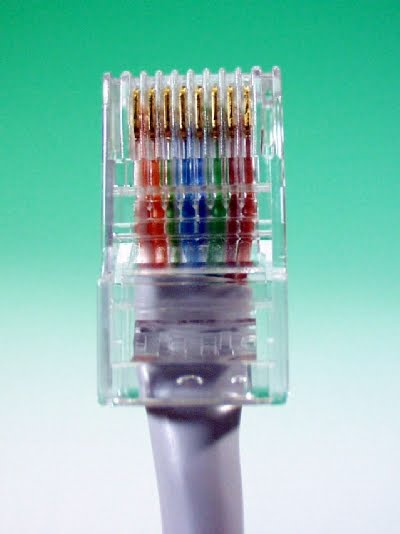
\includegraphics[width=0.2\textwidth]{media/csavart.jpeg}
    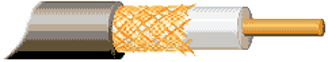
\includegraphics[width=0.33\textwidth]{media/koax.png}
    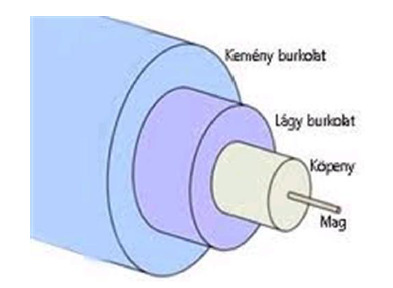
\includegraphics[width=0.33\textwidth]{media/opt.png}
    \caption{\textbf{A legelterjedtebb vezetékes hálózati közegek.} Balról jobbra haladva: csavart érpár, koaxiális kábel, optikai kábel.} 
    \label{fig:vez}
    \end{center}
\end{figure}

\item Vezeték nélküli: Nem mindig megoldható/kényelmes vezetékes hálózat kiépítése. Ekkor számos vezeték nélküli technológia alkalmazható:
\begin{itemize}
\item[-] infravörös kommunikáció kisebb távolságra 
\item[-] rövidhullámú, rádiófrekvenciás átvitel (WiFi, Bluetooth) kisebb távolságra 
\item[-] mikrohullámú átvitel, mely működésének feltétele, hogy a két antennának látnia kell egymást 
\item[-] lézer, műhold
\end{itemize}
\end{itemize}

\subsection {TCP/IP hálózati architektúra}
A manapság legelterjedtebb hálózati architektúra a TCP/IP modell, amely az Internet hivatkozási modellje is. Az architektúra két legfontosabb protokollja a TCP és az IP. A modellben az információ ún. datagramban (csomag) terjed. A TCP (Transmission Control Protocol) végzi el az üzenetek feldarabolását csomagokra az egyik oldalon, míg a másik oldalon a beérkező datagramokból összerakja az eredeti üzenetet. Ez a szint kezeli az esetlegesen elvesző csomagok újrakérését és a sorrendváltozást. Az IP (Internet Protocol) az egyedi datagramok továbbításáért felelős, amely bonyolult lehet amennyiben több hálózaton kell azt keresztül küldeni. Az összes kapcsolat és a különböző vonalak (esetlegesen különböző fizikai hordozókon) kezelése komplex feladat.
A TCP/IP az ún. catenet modellt használja. Ez feltételezi, hogy sok egymástól független hálózat van összekötve egymással. A csomagok ekkor több különböző hálózaton is keresztülmehetnek, mielőtt célhoz érnének. Ez a folyamat a routing, ami a felhasználó számára teljesen láthatatlan. A csomag a célgép Internet címével van ellátva, ami egyértelműen megadja a végcélt. Az internet cím egy 32-bitesszám, amit gyakran 4 decimális számmal jelölnek (IP-cím).  Az egyes gépeken futó eljárások külön-külön is kiépíthetnek TCP/IP kapcsolatot , ezeket egy IP-címen belül az ún. portszámmal különböztetjük meg. Az IP-cím és a portszám együtt egyedi kombinációt alkot, pl.: 128.6.4.194:9999. 
\\ \par
A teljes TCP/IP modell a következő négy rétegből áll (\ref{fig:tcpip}. ábra) :
\begin{itemize}
\item Kapcsolati réteg (link layer): Az aktuális hálózati hardverhez kapcsolódó réteg. Biztosítja az adatok fizikai átvitelét, pl.: Ethernet.
\item Hálózati réteg (internet layer): A réteg biztosítja a datagrammok átvitelét a két gép közötti hálózaton. Ennek a feladata a csomagok az útvonalkijelölése (routing), pl.: IP.
\item Szállítási réteg (transport layer): A két végpont közötti adatátvitelt biztosítja: adatokat fogad a felette lévő rétegből, majd azokat a hálózaton szállítható méretre darabolva átadja a hálózati rétegnek. A célhost oldalon a feladata a beérkező csomagok eredeti sorrendbe rendezése, pl.: TCP, UDP.
\item Alkalmazási réteg (application layer): a felhasználó által indított program és a szállítási réteg között teremt kapcsolatot. Ha egy program hálózaton keresztül adatot szeretne küldeni, az alkalmazási réteg továbbküldi azt a szállítási rétegnek, pl.: FTP.
\end{itemize}

\begin{figure}[H]
    \begin{center}
    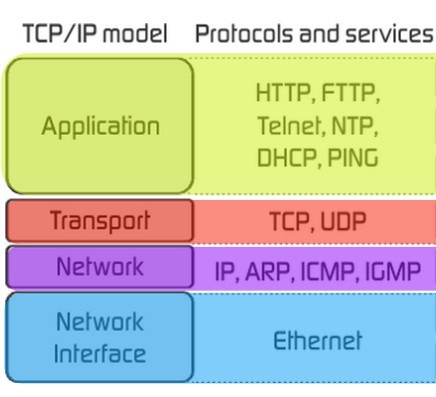
\includegraphics[width=0.35\textwidth]{media/tcpip.jpeg}
    \caption{\textbf{A TCP/IP modell sematikus ábrája.}} 
    \label{fig:tcpip}
    \end{center}
\end{figure}


\subsection {Egyéb protokoll - UDP}
Bizonyos alkalmazások esetén nem szükséges a TCP szintet használni, mivel az üzenet belefér egy datagramba. Ilyen lehet pl.: a név szerinti internetcím keresés. Ilyen típusú célokra az UDP (User Datagram Protocol) használatos. Az UDP a TCP-hez hasonlóan saját port címekkel rendelkezik, és a saját headerjével ellátott csomagot adja át az IP-nek továbbításra. Az IP a távoli gépen nem a TCP, hanem az UDP protokoll kezelő programnak továbbítja a csomagot.

\section{Hálózatok szolgáltatásai}

Amikor az Internet, mint TCP/IP hálózat szolgáltatásait használjuk, a valóságban nem közvetlenül számítógépek kommunikálnak más számítógépekkel, hanem számítógépeken futó programok kommunikálnak más számítógépeken futó programokkal. 
\par
Az Internet a kliens/szerver modell alapján működik. Amikor tehát az Internet szolgáltatásait használjuk, akkor tulajdonképpen két programot veszünk igénybe: a klienst és a szervert. A kliensprogram az, amelyik a lokális terminálunkon fut, ez a program jeleníti meg képernyőnkön az információkat, fogadja a billentyűleütéseket és az egérrel végrehajtott műveleteket, valamint visszakeresi az igényelt információt a szerveren. A szerverprogram abban a számítógépes rendszerben fut, amelyik a szolgáltatást biztosítja.
\par
Számos ilyen hálózati szolgáltatás (szerver) létezik, mint pl.: fájl, webszerver, adatbázis, FTP. Ide tartozik még a tétel tematikájából a
 DNS (Domain Name Server). A programok képesek hivatkozni számítógépre, weboldalakra, email címekre és más erőforrásokra az IP-címek a felhasználásával. Ezek a címek azonban embereknek nehezen olvashatók, továbbá ha egy weboldal egy adott címen van, majd a webszerver átkerül egy eltérő IP-című másik számítógépre, akkor mindenkinek meg kell mondani az új IP-címet is. Ezért magas szintű, olvasható neveket vezettek be, hogy különválasszák a gépek neveit a gépek címeitől, a DNS szerver pedig ez a fordítást végzi a nevek és címek között: www.example.com $\leftrightarrow 192.0.32.10$.

\section{Hálózati eszközök}

Számos egyéb létező hálózati eszköz mellett a tematikában szereplők:
\begin{itemize}
    \item Végpontok: Fizikai pont, amelyen keresztül az előfizető hozzáfér vagy hozzáférhet az elektronikus hírközlő hálózathoz. Kapcsolással vagy irányítással működő hálózatok esetén a hálózati végpont azonosítására egyedi, az előfizetői névhez vagy címhez kapcsolható hálózati cím szolgál. A korábban említett transpont layer biztosítja az adatátvitelt közöttük TCP/IP hálózati protokoll esetén.
    \item Kapcsolók (switch): LAN nagyobb részeit összekötő, több porttal rendelkező eszköz. Két különböző LAN technika (pl. FDDI és Ethernet, vagy két különböző sebességű ethernet) között csak switch-el lehet LAN összeköttetést létrehozni. 
    \item Útválasztok (router): Feladata két hálózatot közötti út kiválasztása, tehát a hálózatok összekapcsolása hálózati szinten. Vizsgálja a címzést, és csak a két hálózat közötti átmenő forgalmat bonyolítja le. Képes lehet topológiai (hálózat változása) és protokollbeli változások követésére (pl.: DECNET és TCP/IP). \par
    Előfordulhat hogy valaki két vagy több ugyanolyan IP címtartományú hálózatot szeretne működtetni, de az elérhető IP címek száma véges és drága is. Ennek megoldására szolgálnak a privát tartományok: ezeken belül tetszőleges számú cím használható, azonban a tartomány határán lévő routereknek nem szabad "ráengedni" az ottani gépeket, a címek lehetséges azonossága miatt.
    A NAT (Network Address Translation) protokoll az ilyen privát tartományokban lévő letiltott hálózatok internethez való kapcsolódását oldja meg címfordítással. Címfordítás esetén a router úgy viselkedik, mintha ő, a megfelelő alhálózatba belógó lábával indította  volna  el  a  kérést - azaz  kicseréli  a  forrás  IP  címét  a  saját,  megfelelő  IP címére (\ref{fig:nat}. ábra).
    
    \begin{figure}[H]
    \begin{center}
    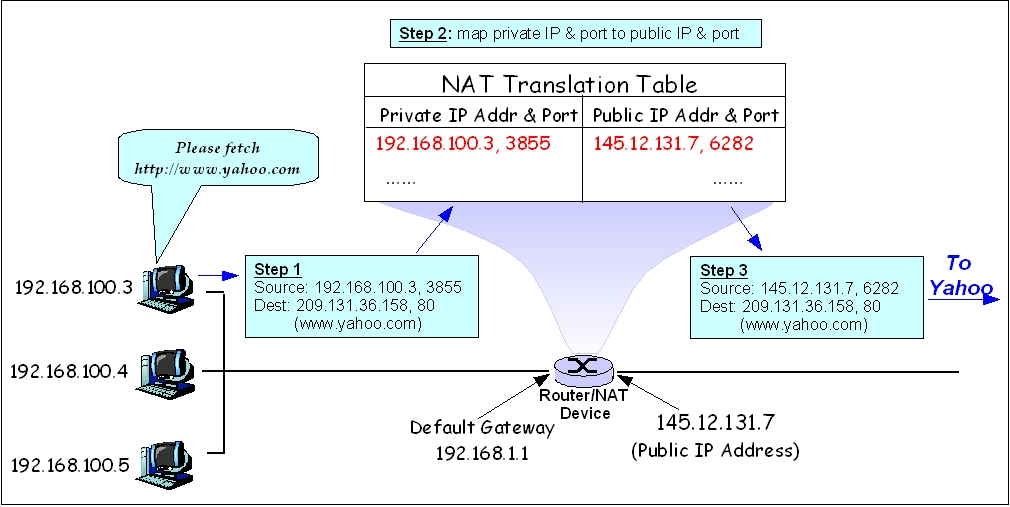
\includegraphics[width=0.90\textwidth]{media/nat.jpg}
    \caption{\textbf{NAT címfordítás.}}
    \label{fig:nat}
    \end{center}
\end{figure}
    
    \item Tűzfalak: a számítógépek összekapcsoltságából természetes módon adódnak adatbiztonsági problémák, illetve rosszindulatú támadások  veszélye. A tűzfal egy csomagszűrőként viselkedik, az adatcsomagok egyszerű szűrése a cél-port, valamint forrás- és célcím, egy a tűzfal-adminisztrátor által már definiált szabályrendszer alapján történik: pl.: egyes portok blokkolása. Nem minden portot lehet blokkolni a kommunikáció teljes elvágása nélkül, erre megoldás a DMZ (DeMilitarized Zone – demilitarizált övezet). A DMZ a  hálózat olyan része, mely kívül esik a biztonsági határon (\ref{fig:dmz}. ábra). Ide bármilyen forgalom bejöhet. A demilitarizált zónában elhelyezett gépeket, pl. egy webszervert, az internethez csatlakozó gépek elérhetik, a belső hálózat weboldalát böngészhetik. Ezek után a tűzfalat be lehet úgy állítani, hogy blokkolja az adott portra irányuló bemeneti forgalmat, vagyis az internetről a belső hálózat gépei nem támadhatók ezen a porton. Hogy a webszerver menedzselhetőségét lehetővé tegyük, a tűzfalnak lehet olyan szabálya, amely megengedi a webszerverhez kapcsolódást a belső gépekről.
\end{itemize}{}

    \begin{figure}[H]
    \begin{center}
    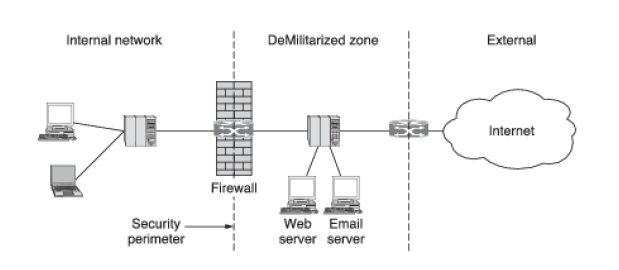
\includegraphics[width=0.75\textwidth]{media/dmz.png}
    \caption{\textbf{Demilitarizált övezet - DMZ.}}
    \label{fig:nat}
    \end{center}
\end{figure}


\section{Sorbanállás, torlódás}

Amikor túl sok csomag van jelen a hálózatban (vagy egy részében), a teljesítőképesség visszaesik, a csomagküldés pedig késleltetést szenved. Ezt a helyzetet torlódásnak nevezzük. A hálózati és a szállítási réteg megosztja a torlódáskezelés felelősségét. Amikor torlódás lép fel a hálózatban, a hálózati réteg ezt közvetlenül érzékeli, és neki kell meghatározni végül, hogy mi történjen a többletcsomagokkal. A leghatékonyabb módszer azonban a torlódás szabályozására, ha csökkentjük a szállítási réteg által a hálózatra rótt terhelést. Ez a hálózati és a szállítási réteg együttműködését igényli (\ref{fig:torl}. ábra).


    \begin{figure}[H]
    \begin{center}
    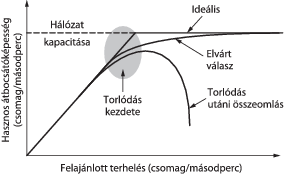
\includegraphics[width=0.4\textwidth]{media/torlodas.png}
    \caption{\textbf{Torlódás: túl nagy forgalom esetén a teljesítőképesség meredeken visszaesik.} Amikor a hosztok által a hálózatba beadott csomagok száma a hálózat átviteli kapacitásán belül marad, akkor minden csomag kézbesítésre kerül (kivéve egy párat, amely az átvitel során hibákat szenvedett), és a kézbesített csomagok száma arányos az elküldött csomagok számával. Ahogy azonban az átvitelre szánt (felajánlott) terhelés eléri a hálózat átviteli kapacitását, a forgalmi löket alkalmanként megtölti az útválasztók puffereit és néhány csomag elveszik. Ezek az elveszett csomagok felemésztik a kapacitás egy részét, így a kézbesített csomagok száma az ideális szint alá csökken. A hálózaton torlódás alakul ki.}
    \label{fig:torl}
    \end{center}
\end{figure}

\section{Adattitkosítás}

Egy hálózat biztonságát nehéz definiálni, azonban mégis alapvető elvárás a felhasználóktól. A hálózat mindegyik protokollrétegéhez hozzátartozik valamilyen hálózati biztonsági mód. A fizikai rétegbeli biztonságot leszámítva minden eljárás valamilyen kriptográfiai elveken alapszik. Példák adatbiztonsági eljárásokra a különböző rétegekben:

\begin{itemize}
    \item A fizikai rétegben a vezeték megcsapolását meghiúsíthatjuk a vezetéknek lepecsételt és argon gázzal feltöltött csőbe helyezésével. Minden kísérlet, amelynek során a csőbe szeretnének hatolni, a gáz elszökésével, és így nyomáscsökkenéssel jár, ami riasztást válthat ki.
    \item Az adatkapcsolati rétegben kétpontos vonalon haladó kereteket kódolással titkosíthatjuk, amikor elhagyja az egyik gépet, és a titkosítást visszakódolhatjuk, visszafejthetjük, amikor a keret a másikra megérkezik. Minden lépést elvégezhetünk az adatkapcsolati rétegben anélkül, hogy a felsőbb rétegek tudnának róla. Ennek a megoldásnak akkor jelentkeznek a korlátai, amikor a csomagoknak több útválasztón kell keresztüljutniuk, mivel ekkor mindegyik eszközön vissza kell kódolni a csomagot, sebezhetővé téve az útválasztón belüli támadásokkal szemben. Emellett nem teszi lehetővé, hogy csak egyes kapcsolatokat védjünk (például online vásárlást bankkártyával), másokat pedig nem. Mindezek ellenére az adatkapcsolati titkosítás (link encryption), ahogy a fenti módszert nevezik, könnyen használható bármilyen hálózaton, és gyakran hatásos.
    \item A hálózati rétegben tűzfalakat telepíthetünk, hogy egyes csomagokat a hálózaton belül, vagy másokat azon kívül tartsunk. Az IP-s biztonsági funkciók szintén ebben a rétegben működnek.
    \item A szállítási rétegben teljes összeköttetéseket titkosíthatunk, végponttól végpontig, vagyis alkalmazási folyamattól alkalmazási folyamatig. A maximális biztonság eléréséhez ilyen végponttól végpontig terjedő eljárásokra van szükség.
    \item Csak az alkalmazási rétegben lehet kezelni olyan kérdések, mint például a felhasználók hitelesítése vagy a letagadhatatlanság.
\end{itemize}{}







\bibliographystyle{plain}
\bibliography{references}

\end{document}
